%%%%%%%%%%%%%%%%%%%%%%%%%%%%%%%%%%%%%%%%%%%%%%%%%%%%%%%%%%%%%%%%%%%%%%%%%%%%%%%%
% simulation.tex: Chapter on MC production:
%%%%%%%%%%%%%%%%%%%%%%%%%%%%%%%%%%%%%%%%%%%%%%%%%%%%%%%%%%%%%%%%%%%%%%%%%%%%%%%%
\chapter{Simulation}
\label{chapter:ldmx:simulation}
%%%%%%%%%%%%%%%%%%%%%%%%%%%%%%%%%%%%%%%%%%%%%%%%%%%%%%%%%%%%%%%%%%%%%%%%%%%%%%%%

\ac{ldmx} (like many other HEP experiments) uses an intricate software stack in order to realistically and efficiently simulate particle interactions with the detector, emulate the electronics that would be used to measure these interactions, and reconstruct the output of these electronics into physically-understandable variables.
These software tasks are accomplished by a wide swath of different software packages, some of which custom-written for \ac{ldmx}, most of which written in C++.
This chapter is focused on describing this simulation infrastructure -- focusing particularly on parts of the infrastructure I was involved in -- while also pointing out areas that are expected to remain constant in the presence of data gathered from a real detector.

\section{General Data Process}
One of the core principles helping organize HEP data is the concept of an ``event.''
Events are a bit abstract to define in terms of the physical experiment; however, they are slightly easier to define within the confines of our data processing software.
In essence, each event within the software is independent from one another however they all share a similar structure to the information they hold. A natural example is a data table: a row has the same values in each of its columns as all the other rows. Events behave the same way; however, unlike a data table, the structure of an event can be more intricate than simply a series of values corresponding to different column titles.
While our basic ``unit'' of data is an event, we require many events in order to make statistical conclusions about our data; thus, we have developed a ``event processing framework'' that allows us to unify the various aspects of processing the data held within an event.

\begin{figure}
    \centering
    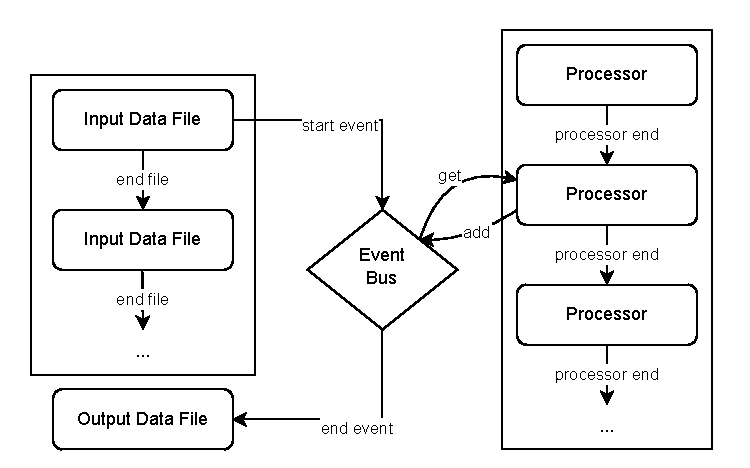
\includegraphics[width=0.9\textwidth]{figures/ldmx/simulation/FrameworkFlowChart.drawio.pdf}
    \caption{Flow chart of how data is processed in the \ac{ldmx} framework. Each processor has the ability to ``add" data to the event as well as ``get" data from the event. The processors are run in a user-defined sequence. Data can also be loaded from one or more input data files where the event data from those files is loaded into memory before the first processor is run. After all processors are done with an event, it is saved to the output data file.}
    \label{fig:ldmx:sim:data-flow}
\end{figure}

The event processing framework designed, developed, and maintained by \ac{ldmx} is focused on allowing for the flexibility necessary to do the wide range of tasks necessary for the experiment. The C++ framework uses CERN's ROOT \cite{cernroot} for data serialization, Boost \todo[citation]{need a citaiton for Boost libraries} for logging, and Python \cite{python} for dynamic run-time configuration. The design is a sequential model: each ``event" is passed to individual processors in a certain sequence. The individual processors can put data ``into" the event for later processors to use and eventually serialized into the output ROOT file. The processors can be built separately from the framework and then dynamically loaded and created at run-time by an abstract factory. This design choice allows for all of the computationally-intensive software tasks necessary for \ac{ldmx} (simulation, reconstruction and some analysis tasks) to use this framework and be organized into separate modules which are only loaded into memory when that module is being used.

The serialization portion of the framework is similarly dynamic; focusing on enabling users' code to add data structures from the most simple (e.g. individual booleans) to the most complicated (e.g. containers of custom classes). This wide array of data types is supported by ROOT's dictionary system during the serialization stage and abstract wrapper classes with partially-specialized template derivatives during run-time. This complexity within the framework is necessary in order to allow a simple interface -- one where the user interacts with simple and complex types in the same way.

Combining this highly dynamic serialization library with the sequential-processing model configured at run-time gives a strong foundation for all of the software needs of \ac{ldmx}. Written in C++, this software framework enables high performance for all of the major data processing tasks necessary for the experiment. Moreover, its design focuses on flexibility and modularity so that seemingly disparate data processing tasks can be unified under one framework. Everything from simulation to detector emulation to event reconstruction to analysis calculations can be done within this framework, reading and writing files from this framework and enabling our software to be well organized while also centralized in one location.

\subsection{Data Processing Stages}
The centralized nature of the \ac{ldmx} processing framework makes it much simpler to stay unified as a collaboration. Experts are allowed to work on their specialized area of the software and shares those improvements with the entire collaboration with ease. Since the flexibility of the framework allows for arbitrary groupings of these different data processing stages, we can choose to separate them into natural groups that correspond to the different areas on which experts focus (diagrammed in \cref{fig:ldmx:sim:data-stages}).

\begin{figure}
    \centering
    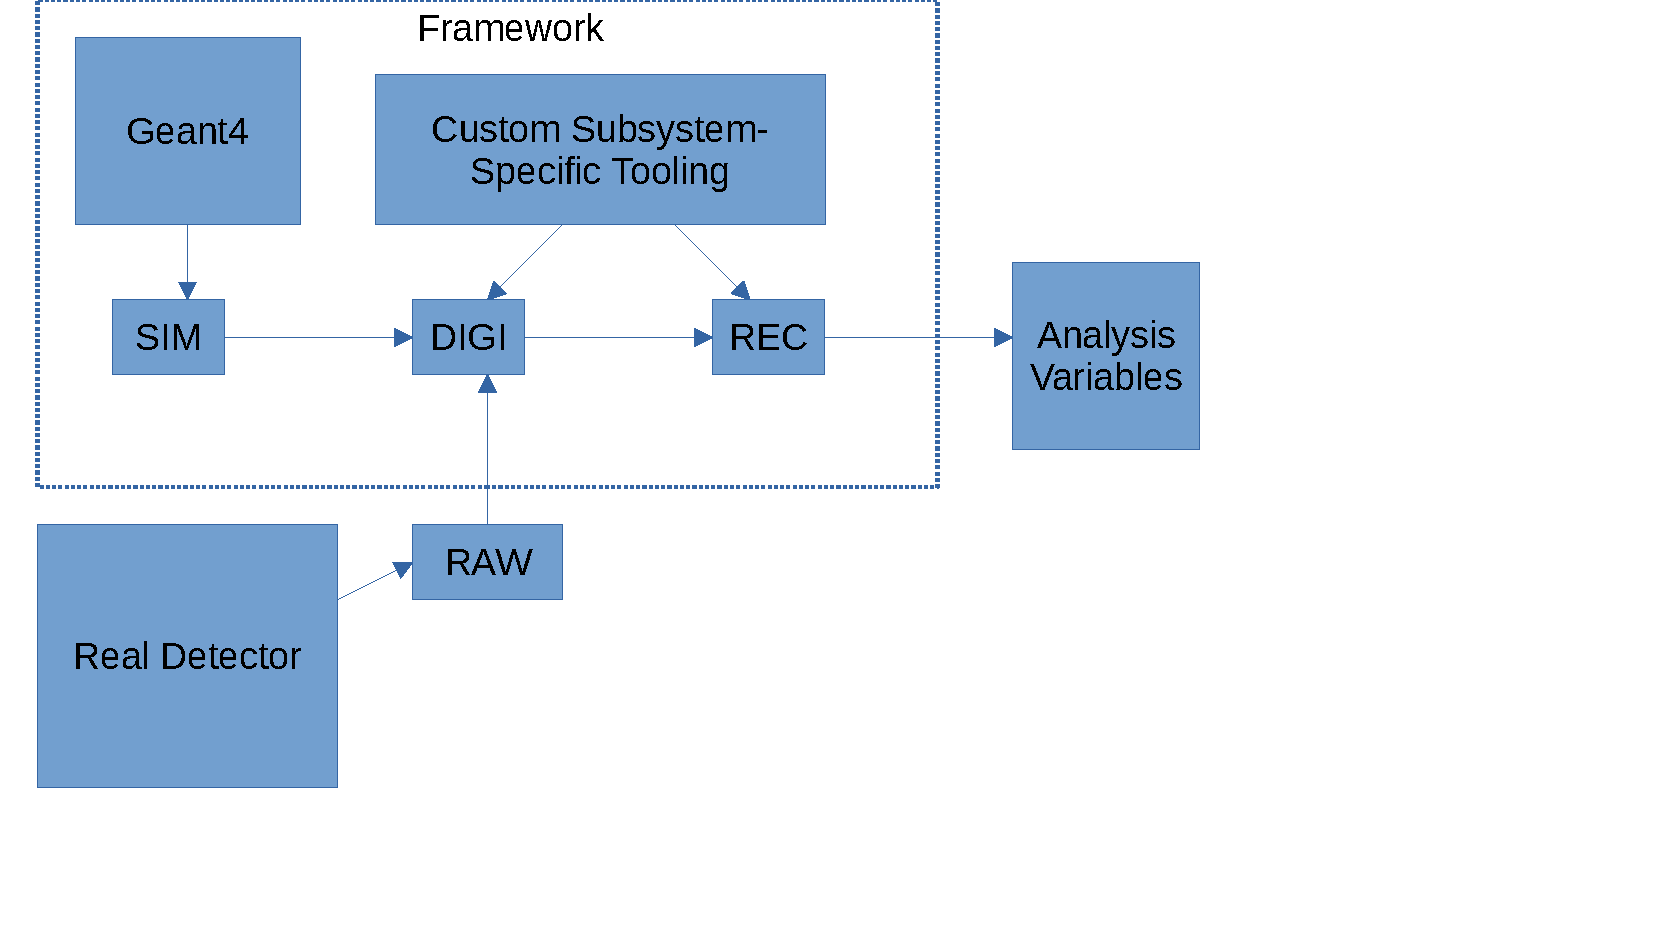
\includegraphics[width=0.9\textwidth]{figures/ldmx/simulation/data-flow.pdf}
    \caption{Diagram of processing stages within \ac{ldmx} showing the external sources of data or software that are used in those stages as well as which stages are commonly done within the centralized processing framework.}
    \label{fig:ldmx:sim:data-stages}
\end{figure}

In this work (as the chapter title implies), we focus mainly on the detector simulation stage where data is randomly generated in a way geared towards realistically modeling the detector and particles interacting with it. The downstream stages, namely electronic emulation and reconstruction, are not described further here; however, it should be emphasized that all subsystems of \ac{ldmx} have their own custom implementations of these stages in order to realistically emulate and reconstruct the data within their subsystem.

\section{Standard Processes}
As displayed in \cref{fig:ldmx-bkgd-staircase}, there are a few categories of physics processes that are described by the standard model and we expect to happen within our experiment. These ``background'' processes -- while interesting for other analyses of \ac{ldmx} data -- should be rejected by this search for \ac{dm} since they are understood to \emph{not} be \ac{dm} by the standard model and other experiments. In order to thoroughly and faithfully estimate our ability to reject these backgrounds, we need to realistically simulate them within our detector volume.

\textsc{Geant4} \cite{geant4} has been developed for precisely this purpose. This study uses a slightly modified copy of \textsc{Geant4} v10.2.3 which focuses on improving the accuracy of processes relevant to a \ac{dm} search within \ac{ldmx}.
\begin{enumerate}
    \item Updating cross section and sampling of $\gamma\to\mu^+\mu^-$ process to align it better with collected data and calculations of the standard model.
    \item Update nuclear cascade to align with more recent CLAS data specifically focused on the rate of low-multiplicity forward neutrons (Appendix A.A of \cite{ldmx-whitepaper}).
    \item Introduction of \emph{back scattering} $\pi^0$ in a $\gamma p \to \pi^0 p$ within a nuclear cascade (Appendix A.B of \cite{ldmx-whitepaper}).
\end{enumerate}
These updates enabled us to efficiently study the known and expected background processes interactions with the \ac{ldmx} detector design and compare this data to simulations of a model of a \ac{dm} production process.

\subsection{Biasing and Filtering}
Biasing and filtering methodology, configuration for EaT-specific backgrounds.
\todo[copy]{Copy MidShower Parameters appendix from EaT internal note.}

\subsection{Validation}
Validation of this methodology.
\todo[copy]{Copy background sample validation appendices from EaT internal note.}

\section{Dark Matter Signal}
The particular signal process this analysis channel is looking for is the
production of a dark photon followed by an \emph{invisible} decay. In this
regime, what happens to the dark photon after it is produced is irrelevant
to the analysis since both it and its products are not observable by our
detector.

With this focus in mind, we developed a dark bremsstrahlung simulation method
that allows for the visible particle (the recoiling lepton) to be distributed
according to a full matrix element calculation (via MG/ME) while the incident
particle can have varied energy and be handled by Geant4 directly. This novel
simulation technique allows for the dark bremsstrahlung process to be treated
(from Geant4's perspective) on the same footing as the background processes
while maintaining the precision of a matrix-calculator method.

\subsection{G4DarkBreM}
To accurately simulate the kinematics of the dark bremsstrahlung process for electrons in thick targets, the process must be included at the level of experimental simulation instead of using initial state event generators to account for the possibility of energy loss through bremsstrahlung or multiple scattering prior to the dark matter interaction. Accurate kinematic simulation of the outgoing electron are required for optimal experimental sensitivity measurements and appropriate design of search strategies.

For this reason, we utilize G4DarkBreM \cite{g4darkbrem} which performs this embedding of the dark bremmstrahlung process into \textsc{Geant}4. G4DarkBreM calculates the cross section using numerical integrals of the Weizs\"{a}cker-Williams approximation, and the kinematics are simulated using a scaling technique of \textsc{MadGraph/MadEvent} event libraries. The accuracy of the total cross section and kinematics is validated using \textsc{MadGraph/MadEvent} samples.

\subsection{MadGraph/MadEvent}
Detail on MG/ME workspace used to generate DB libraries.

\subsection{Characterization}
Describe how these samples "look"?

%%%%%%%%%%%%%%%%%%%%%%%%%%%%%%%%%%%%%%%%%%%%%%%%%%%%%%%%%%%%%%%%%%%%%%%%%%%%%%%%
